\section{Introduction}\label{sec:intro}
Textual program editors are powerful and expressive user interfaces, 
so it is little wonder that they remain dominant decades after the teletype. 
However, textual user interfaces are not the best tool for every job. 
In particular, there are many 
data types for which a non-textual  
user interface may situationally be more appropriate \cite{Graphite}.

For example, consider the following record type%
\footnote{We will assume that we are in an ML-family language, 
e.g. Elm \cite{Elm,ElmArchitecture,czaplicki2012elm}, 
for the remainder of this paper, though the ideas are general.} 
classifying colors using an RGBA encoding:
\begin{lstlisting}[numbers=none]
type Color = { r: Int, g: Int, b: Int, a: Int }
\end{lstlisting}
It is possible to select a particular color by entering  
an expression of this type using a text editor:
\begin{lstlisting}[numbers=none]
let bgcolor : Color = { r: 255, g: 178, b: 45, a: 100 }
\end{lstlisting}
The problem is that this \emph{de facto} user interface for color selection 
offers the user no immediate feedback 
and limited editing affordances.
It is difficult for the programmer, or anyone subsequently reading the code, to know which color is represented 
and to interactively tweak that color. 
Better support for activities like these would be particularly helpful when engaging in 
live and exploratory programming in domains like web design, audio-visual production, 
and interactive data analysis.

Indeed, practitioners in domains like these commonly eschew general-purpose programming 
in favor of graphical end-user applications, like %
image and video editors, spreadsheets, and music composition software, 
that do provide live feedback and 
direct manipulation affordances, e.g. color palettes, visual timelines, and interactive plots. 
The trade-off is that these end-user applications have limited support for abstraction and composition. 
It is difficult, for example, to bind a
color to a variable for use in multiple locations, 
or to compute a darkened color by passing it to a function, 
or to organize and distribute color schemes using a package manager.
Moreover, it is difficult to compose affordances in ways that the application designer has not 
anticipated, 
e.g. to use a slider to manipulate the alpha channel 
if the native color palette provides only a text box\todo{better example?}{}.

This paper aims to resolve this apparent tension between 
programmatic and direct manipulation interfaces by designing a programming system that 
is able to surface GUIs when working with the data types for which 
they are useful, while retaining support for textual program manipulation  
and the full array of abstraction and composition mechanisms
available in modern general-purpose programming languages.

\subsection{Background}
\begin{figure*}
  \begin{center}
  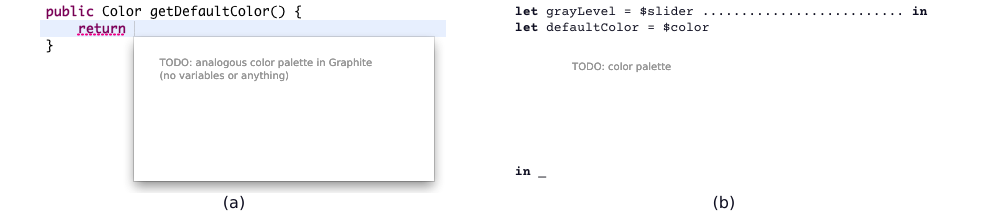
\includegraphics[width=35pc]{color-palettes.png}\end{center}
  \caption{
  (a) This figure, adapted from the prior work of \citet{Graphite}, 
  shows a Graphite palette associated with the \texttt{Color} class. 
  The client can specify the RGBA components only using literal numbers. 
  (b) A similar Hazel livelit for colors uses live splices for the RGBA components,
  so the client can enter any Hazel expression. 
  In this case, the client has entered a variable into the RGB 
  splices, which itself was defined using a slider livelit. 
  The livelit can evaluate splices under its closure to display the 
  computed color. 
  The value of \li{defaultColor} is determined by the livelit via a macro expansion step.}
  \label{fig:color}
\end{figure*}

We are not, of course, the first to integrate direct manipulation user interfaces
into general-purpose programming systems.
Prior work on projectional editing
and active code completion, summarized in Sec. \ref{sec:related-work}\todo{sections}{}, 
has also considered the problem of entering expressions 
of certain types, like \li{Color}, 
using specialized GUIs integrated into the editor. 
The prior work most closely related to this paper is the {Graphite} system for Java \cite{Graphite}.
Graphite allows library providers to associate a GUIs, called \emph{palettes}, with types (using Java's class annotations). 
Wherever an expression of a type equipped with a palette is needed, 
i.e. wherever there is a \emph{hole} of that type in the program, 
the programming environment offers the programmer the option, via the code completion menu (not shown), 
to activate the palette. 
It is the palette's job to generate an 
appropriate expression to fill the hole once the interaction is finished. 
Figure~\ref{fig:color}(a)\todo{use subfigure?}{}, adapted from this prior work, demonstrates a simple color palette.
When the user presses the \li{Enter} key, the Java code \li{new Color(0, 0, 128)}\todo{correct code}{} is inserted at the cursor (not shown) and the palette disappears.

\citet{Graphite} extensively evaluated this mechanism. 
Most notably, a survey of approximately 450 developers found that 
most developers viewed the proposed mechanism favorably and stated that they 
would use a suitable palette some or all of the time if one was available.%
\footnote{When presented with a color palette, 
many participants remarked that they rarely entered colors directly into Java code, 
but rather into stylesheets or other files governed by a domain-specific language. 
Other palettes, e.g. a palette
that supported regular expression construction and testing, were viewed as more 
suitable for Java code. 
The mechanisms being considered are suitable both for general-purpose languages
and typed domain-specific languages, many of which can be embedded into modern 
general-purpose languages, e.g. Typed CSS in Reason. TODO: CITE}

This survey also solicited a large number use cases from the survey participants, 
which the authors grouped into several broad categories. Notable examples include:
\begin{itemize}
  \item \textbf{graphical elements}, such as brushes, fonts, polygon editors, user interface widgets, and 3D primitives;
  \item \textbf{data analysis primitives}, such as plot setups and database queries; 
  \item \textbf{data structures} such as matrices, maps, queues, and others for which specialized notation (e.g. JSON) may be more suitable than general-purpose notation; and
  \item \textbf{data transformations} for which sensory feedback could aid in understanding, 
  e.g. audio filters, image transformations, and animations with parameters such as speed and shape.
\end{itemize}

We take this extensive empirical evaluation as sufficient to establish 
the utility and broad applicability of a mechanism of this sort. 

\subsection{Contributions}

Our focus in this paper is on addressing several non-trivial technical 
deficiencies that limit both palette providers and palette clients in Graphite. 
The system of \emph{live literals}, or \emph{livelits}, introduced in
this paper and demonstrated in Fig.~\ref{fig:color}(b), differs from Graphite  
in each of the following ways.
\begin{enumerate}
  \setlength\itemsep{0.5em}
  \item \textbf{Decentralized Extensibility}: 
    Graphite allows only the provider of a type to define a corresponding palette. 
    By contrast, livelit definitions are orthogonal to type definitions. 
    Clients invoke livelits explicitly by name (names are prefixed by the \li{\$} symbol, 
    e.g. \li{\$color} and \li{\$slider} in Fig.~\ref{fig:color}(b)).
    We call this \emph{decentralized extensibility}.
  \item \textbf{Persistence}: Graphite's palettes are {ephemeral}, 
  i.e. they disappear after the initial interaction, 
  leaving behind only the generated textual code.%
  \footnote{Graphite does include an \emph{ad hoc} mechanism that 
  allows palettes to parse the code that is selected in the editor 
  when the palette loads, but this requires that each palette implement 
  a parser for the subset of Java used in the code that it generates,
  and therefore this mechanism is quite brittle. It is also difficult 
  to persist GUI state that is not included in the generated code.}
  Consequently, only the programmer that initially enters the expression 
  benefits from the feedback and affordances that the palette provides.
  By contrast, livelits are persistent. We use a pure functional model-view-update architecture 
  (i.e. the Elm architecture\todo{what to cite?}{}) as our GUI framework, 
  so only the model needs to be persisted, rather than the full GUI state.  
  We use the word ``literal'' rather than ``palette'' because, with persistence, livelits
  are more analogous to literal notation, e.g. list literals.

  \item \textbf{Compositionality}: 
  Graphite does not provide any way to {enter subexpressions within a palette}.
  At best, palettes can contain text boxes, but expressions entered into these text boxes 
  do not have any editor support (which creates many problems, one of which is that they cannot themselves be generated by palettes). 
  This implies that palettes can only reasonably generate {closed expressions}. 
  For example, in Figure~\ref{fig:color}(a), the color palette
  is useful only for generating simple color constants. 
  By contrast, livelits have first-class support for subexpressions, which we call \emph{splices} (following
  the terminology of \citet{TLMs} who developed reasoning principles for splicing in a purely textual setting).
  Fig.~\ref{fig:color}(b) demonstrates splicing: the client is able to define a variable, \li{grayLevel}, 
  to capture the relationship between the red, green, and blue components.
  The client is also able to use a slider inline in the splice governing 
  the alpha (A) component.
  \item \textbf{Liveness}: Graphite's palettes do not have 
  access to the run-time environment. By contrast, livelits can evaluate splices
  and therefore provide feedback related to the run-time behavior of the expression being generated. 
  For example, in Fig.~\ref{fig:color}(b), the color that is displayed is determined by evaluating the RGBA 
  component splices to numeric values.
  Evaluation occurs in a run-time environment (i.e. closure) determined by 
  leaving the hole being filled by the livelit temporarily unfilled and then evaluating
  using a two-phased variation on the semantics for incomplete programs developed by \citet{HazelnutLive}. 
  We will see more sophisticated examples later in the paper, including a livelit 
  that appears inside a function that is called multiple times, leading to multiple closures for the client 
  select from.
  \item \textbf{Parameterization}: 
    \cyrus{... this would be really nice to include + demonstrate with slider bounds and later data flow + 
    we need it to do anything non-trivial with hygiene 
    ...}
\end{enumerate}
\clearpage

The remainder of the paper is organized as follows. We begin in Sec.~2 with two case studies 
involving several non-trivial livelits, focusing on the client programmer's perspective. 
We then consider the livelit provider's perpsective in Sec.~3.
In Sec.~4, we provide a formal account of the mechanism as a typed lambda calculus. 
This calculus formally specifies the essential aspects of livelit representation and 
the livelit expansion process, independent of the particularities of our implementation, 
and establishes essential type safety and hygiene properties. 
In Sec.~5, we describe some extensions of the core mechanism\todo{what are the extensions?}{}.
In Sec.~6, we outline our implementation of livelits within Hazel.
In Sec.~7, we situate livelits relative to other related work. 
Finally, we conclude in Sec.~8 with a discussion of some present limitations and future work.\todo{section refs}{}

\section{Case Studies}
\subsection{Hazel Overview}
Brief overview (1/2 page) on Hazel (what do holes look like? structure editing, but not in too much detail,
live evaluation)

\subsection{Live Grading}
\subsubsection{Overview}
Talk about the scenario

Live matrix: what is a matrix structurally? (data frame? list of lists?) + how does liveness work
+ overview of hygiene guarantees

Grade cutoffs: how does it work wrt liveness? (do we use a parameter here instead of a splice?) -- 
focus on domain-specific benefits here.

\subsection{Image Transformation Pipeline}
Show example of an image transformation pipeline going through livelits

This might also benefit from Parameterization

Show multiple calls with different example images + closure selector UIs

Go into more detail about how evaluation works + fill-and-resume mechanics (and efficiency nod)

Talk about probes?

\subsection{Additional Examples}
It would be nice to have a gallery-style figure and a brief overview of some other case studies
and how they exercise the novel features of the livelits mechanism. Maybe some statistics on how
many lines of code it took.

\section{Livelit Definitions}
Which livelit implementation do we want to show? Maybe grade cutoffs? Slider as simple intro + color chooser?

Talk about each component of a livelit definition:
\begin{itemize}
  \item livelit name (talk about binding structure)
  \item expansion type
  \item model type (must be serializable)
  \item action type (mention integration into Hazel's undo system)
  \item initial model
  \item update function (monadic actions; talk about color palette update; SpliceRefs)
  \item view function (monadic actions; talk about GUI stuff? tab order? dimensions? mostly defer to Elm for details)
  \item expand function (should we call it fill?)
\end{itemize}

Hygiene from a provider's perspective -- have to use parameters to explicitly capture definition site bindings.


\section{A Typed Livelit Calculus}
Should we talk about anything other than expansion + hygiene, i.e. parameterization, closure collection, closure resumption?
None of that is mechanized, but that may be okay. Closure collection and resumption seem to be worth formalizing.

Note: probably just going to omit the whole livelit function thing

Subsection about Agda mechanization (Ian + Nick?)

\section{Extensions}
Is this section necessary?

\section{Implementation Considerations}
What should we talk about here? Layout of livelits? 

\section{Related Work}
Cyrus has a list somewhere, ask if you want to work on this section

\section{Discussion and Conclusion}
Future work:
\begin{itemize}
  \item pattern matching
  \item type splices
  \item module splices
  \item explicitly make bindings available in splices
  \item better UI for closure provenance / connect with control flow / call stack better
  \item deriving livelits from type definitions
  \item bidirectional evaluation ala SnS
  \item integration with structure editing more cleanly
  \item \dots
  \item collaborative editing?
  \item side effects?
  \item full screening livelits (or compositions thereof) as a way to create end-user workflows
  \item big vision: authoring environment based on livelits
\end{itemize}
\clearpage
\appendix
\section{Misc. Material from Prior Draft}

To address these limitations, we introduce live literals, or livelits. Figure~\ref{fig:cutoffs} shows a mockup of the definition and application of a livelit named \li{$grade_cutoffs} for adjusting grade cutoffs, represented as values of  record type \li{grade_cutoffs}. Like textual literal forms (e.g. list literals), livelits are alternative representations of expressions of the associated type \cite{DBLP:journals/pacmpl/OmarA18}. % From the perspective of the remainder of the program, \li{cutoffs} is a value of type \li{grade_cutoffs} like any other.
We are implementing livelits in Hazel (\url{hazel.org}), a live functional programming environment with support for typed holes \cite{popl-paper}. We plan to perform a live demo.




The definition of
the livelit, outlined in Figure~\ref{fig:cutoffs}, follows the Elm architecture,
i.e. there are types representing the abstract model and the messages that the 
GUI generates. Livelits are \textbf{persistent} rather than ephemeral, i.e. the model is recorded in the underlying syntax tree. The \li{view} function generates the GUI, implemented using HTML, on demand (so the view is not persisted). Another function, \li{to_exp}, is responsible for generating the underlying expression, called the \emph{expansion}, from the \li{model}. 
While other projectional editors, e.g. those generated by Citrus \cite{DBLP:conf/uist/KoM05}, also support persistent GUIs in code, they are not user-extensible. 

The GUI can itself contain typed holes, represented by the \li{HtmlHole} constructor. In this case, there is a single hole
for entering an expression of type \li{list(float)}, i.e. the list of weighted
averages. In this example, the user has filled this hole with a variable,
\li{weighted_averages} (the definition of which precedes the content of this figure and is not shown). In other words,
livelits support \textbf{open expressions} and therefore interact cleanly with 
standard abstraction mechanisms, i.e. they can appear under binders. We follow the reasoning principles for literals with spliced sub-expressions established  by \citet{DBLP:journals/pacmpl/OmarA18}.

The main complication when dealing with open expressions relates to how live feedback
is to be generated. Given just the symbolic expression in the hole, it would be 
impossible to plot (as orange dots) the actual data from the list that the variable refers to. To resolve this issue, the system evaluates the program 
as if it the livelits were empty holes, 
relying on the support for evaluating incomplete programs described recently 
by \citet{DBLP:journals/pacmpl/OmarVCH19}. The result of evaluation is an expression containing
hole closures, i.e. holes equipped with environments. 
%Hazel allows the user to interactively select which closure
%interests them if multiple closures for a given hole appear in the result (e.g. if a livelit appears inside a function called multiple times). 
The livelit 
can then evaluate the expression in the hole against the closure selected by the user (not shown) using \li{Env.run}.


%%%%%

\todo{this is the WIP one from last year}{}
Programs are most often represented as text.
%
This representation format provides expert programmers access to a variety of
text editors and text edit actions---to affect fine-grained control over
programming decisions---and a large ecosystem of other text-based
utilities---for example, for line-based file differencing of source code
versions.
%
On the other hand, the flexibility and low-level nature of text comes at some
costs.
%
For experts, some tedious and manual edits could lead to
inefficiency---especially because many routine code editing operations do not
require the full flexibility of text~\citep{XXX}.
%
For novices, the large class of syntax errors that stem from text-edits presents
a steep learning curve.

Motivated to overcome the disadvantages of represent programs as text, a variety
of alternative code editing interfaces have been investigated.
%
At the opposite end of text are \emph{visual programming languages}, which often
completely represent a program with graphical elements~\citep{XXX}.
%
To forgo text completely, such approaches often target domain-specific
languages, such as dataflow programing~\citep{XXX} and pedagogical languages
that are, by design, restricted to relatively few building blocks.
%
Other \emph{structure}, or \emph{projectional} editors, still use a significant
amount of text to render programs, but forgo text-edits in favor of
\emph{structure edit actions} which transform the program (represented as a tree
or some other structure), sidestepping the danger of invalid intermediate states
of concrete syntax.

On the spectrum somewhere between fully text- and fully structure-based are
``hybrid'' editors, which augment text with additional ways to visualize and
manipulate the structure of the program.
%
Victor Scrubbing, APX~\citep{APX}, Sketch-n-Sketch~\citep{sns-pldi}, and Carbide
IDE~\citep{XXX}, among others, allow numeric values to be ``scrubbed'' by
directly manipulating sliders rather than text-editing numeric literals.
%
Barista~\cite{Barista} is a hybrid Java editor where custom \emph{structure
view} GUIs provide alternate representations of expressions instead of text.
%
For example, an arithmetic expression may be rendered with mathematical symbols,
a method may be accompanied by interactive documentation with input-output
examples, and structures may be selectively collapsed, expanded, or zoomed.
%
Graphite~\citep{Graphite} allows custom GUIs---called \emph{palettes}---to help
the programmer fill missing expressions---``holes''---in the program.
%
For example, a color palette can provide visual previews of different candidate
color values, and a regular expression palette can show input-output examples
for different candidate regular expressions.

The GUI representations and interactions enabled by the above hybrid editors are
useful, but several limitations likely preclude wider utility:
%
the types of expressions that benefit from alternative GUI editors are limited
to
%
privileged types that have baked-in interfaces~\citep{XXX}
%
or just of base type~\citep{XXX};
%
the GUI view is ephemeral, in that it disappears once it has been used to
generate an expression~\citep{XXX}; or
%
expressions generated by the GUI are not deeply integrated with the static type
system and interpreter of the language~\citep{XXX,XXX,XXX}.


%% refactoring
%% 
%% DNDRefactoring~\citep{DNDRefactoring}
%% Deuce~\citep{sns-deuce}


\parahead{Persistent, Composable, and Live GUIs for Filling Holes}

compared to the ``simple'' palettes

extend palettes with: persistence, composition, and live feedback

macro systems allow alternative syntactic (i.e. string) representations, to
expand into underlying expressions

palatable

by analogy to these ``literal'' macro systems, palettes are ``graphical
macros'': through interaction with the user, the GUI generates the underlying
expression.

TLMs~\cite{TLMs}


\parahead{Contributions and Paper Outline}


design for palettes. specifically, within the Hazelnut Live framework,
which is a system to address the gap problem that arises in traditional editor
frontends.

demonstration of the expressiveness of the approach through a series of
examples, many of which are drawn from the user study mentioned before.

a prototype implementation of palettes within Hazel, which currently
supports several examples using a core calculus with minimal features. the
implementation provides a clear path for scaling up to larger, full-featured
syntactic programming conveniences, as well as further UI design in future work.

prototype UIs:

  \begin{enumerate}
    \item \Hazel{}: (palette macros;) structure edit actions; expression formula bar; inline layout
    \item \sns{}: (palette functions;) text editor; pop-up menu
  \end{enumerate}

hazelnut~\citep{Hazelnut,HazelnutLive}



\begin{figure*}[t!]
  \begin{center}
  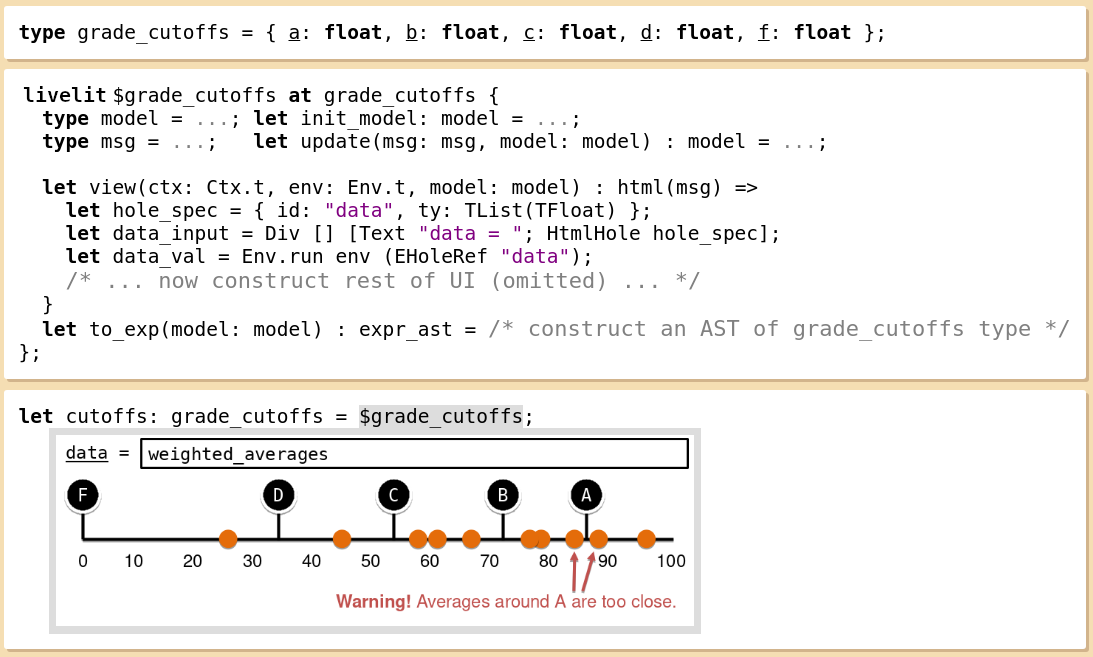
\includegraphics[width=34pc]{cutoffs-mockup.png}\end{center}
  \caption{A mockup of a livelit for adjusting grade cutoffs. Livelits are persistent and can access the live environment.}
  \label{fig:cutoffs}
  \end{figure*}
  